% CS 6604 / ECE 6256 — Assignment 3 report (Gradescope PDF, <= 3 pages incl. AI disclosure)
%
% Build:   cd report && latexmk -pdf main.tex
% Figure:  figures/ablation.pdf is a copy of ablation/results/ablation.pdf.
%          After re-running ablation/plot_ablation.py:  cp ../ablation/results/ablation.pdf figures/
% Numbers: every number in Section 2 comes from ablation/results/*.csv, ablation/mechanism.py,
%          or the paired comparison printed by ablation/run_ablation.py.
%
% Red \todo{...} marks are facts only the team can supply. Search for "todo" before submitting.

\documentclass[10pt,letterpaper]{article}
\usepackage[margin=0.75in]{geometry}
\usepackage[T1]{fontenc}
\usepackage{newtxtext,newtxmath}
\usepackage{microtype}
\usepackage{graphicx}
\usepackage{booktabs}
\usepackage{enumitem}
\usepackage{xcolor}
\usepackage{titlesec}
\usepackage[hidelinks]{hyperref}

\setlist{nosep, leftmargin=*}
\titlespacing*{\section}{0pt}{7pt}{3pt}
\titlespacing*{\paragraph}{0pt}{3pt}{0.6em}
\setlength{\parskip}{2pt}
\setlength{\parindent}{0pt}
\setlength{\textfloatsep}{8pt}
\setlength{\abovecaptionskip}{3pt}

\newcommand{\todo}[1]{\textcolor{red}{\textbf{[TODO:} #1\textbf{]}}}
\newcommand{\code}[1]{\texttt{#1}}

\begin{document}

\begin{center}
  {\large\bfseries Assignment 3: The Course TA-Bot --- Conversational RAG with Memory}\\[3pt]
  Asal Roudbari (aroudbari3@gatech.edu) \quad\textbullet\quad \todo{teammate name, email}
  \\[1pt]{\small CS 6604 / ECE 6256 Conversational AI, Georgia Tech}
\end{center}

% ======================================================================
\section{System: retrieval and generation}

Each \code{chat()} call decides whether to retrieve, retrieves excerpts with BM25, builds a
grounded prompt, calls the course vLLM endpoint, and maps the model's numbered citations to
paper IDs. Every setting comes from \code{config} (with defaults); nothing is hard-coded.

\begin{itemize}
  \item \textbf{Index.} The shipped \code{corpus.db}, unchanged: 108 papers, 5{,}711 chunks of
    ${\approx}400$ tokens (15\% overlap), and its SQLite FTS5 index with Porter stemming. We use
    no embeddings: BM25 is deterministic, fast, and already clears the dev hit-rate bar.
  \item \textbf{Query.} The message's words, minus stopwords and instruction words
    (``explain'', ``paper''), each quoted and OR-joined. Raw text crashes FTS5 on punctuation,
    and FTS5's default AND matches nothing for long questions.
  \item \textbf{Ranking.} BM25 over title and chunk text. We take the top 100 chunks, rank papers
    by their best chunk, keep the top $k{=}3$ papers, and fill 4 excerpt slots breadth-first
    (one per paper, then a second from the strongest): retrieve wide, keep narrow (L13).
    Breadth-first fixed a dev turn where four excerpts from two similar papers crowded out the
    gold paper.
  \item \textbf{Follow-ups.} Each session records the top paper of every turn. A singular
    reference (``it'', ``this method'') carries the previous turn's paper into the excerpts; a
    plural one (``both'', ``the ones we discussed'') carries up to the last three; ``switching
    topics'' carries none. Greetings, thanks and questions about the user skip retrieval.
  \item \textbf{Prompt.} A system prompt tells the model to answer from the excerpts, cite them
    as \code{[n]}, name the paper, say when the excerpts do not cover the question, and keep each
    claim attributed to its own paper. Then come the last 3 exchanges (assistant turns clipped to
    600 characters) and the numbered, titled excerpts (${\le}2{,}000$ characters each), ordered
    best first and second-best last, against ``lost in the middle'' (L13). About 2k tokens.
  \item \textbf{Generation and failures.} OpenAI-compatible \code{/v1/chat/completions} with the
    configured temperature and seed, at most 512 new tokens. Network errors, HTTP errors and
    malformed replies all raise \code{TimeoutError}, as the contract requires.
  \item \textbf{Citations.} \code{[n]} markers become paper IDs in the answer, with adjacent markers
    merged; out-of-range markers are dropped. \code{citations} lists every paper whose excerpt the model saw (3, plus
    carried papers on follow-ups), filtered to valid IDs. This favours recall over citation
    precision, which is why the ablation measures the budget $k$.
\end{itemize}

\textbf{Dev results} on PACE (Llama-3.1-8B-Instruct, vLLM 0.31, one H100): preflight passes;
single-turn hit-rate 10/10; multi-turn 3/3. All 10 turns also hit when every turn is scored; the
harness scores only the last turn, which had hidden a turn-1 miss during development. Across 44
answers there were no errors. Latency averaged 2.3\,s (max 4.5\,s), prompts stayed under 2.2k
tokens, no answer hit the 512-token cap, and a fresh second run reproduced all 10 single-turn
answers exactly. Reading the answers showed three problems, which we fixed and re-ran. Citations
repeated (``[L11-01] [L11-01]'' when two excerpts share a paper), and paper IDs and section names
were copied from the excerpt headers. Merging adjacent markers and showing only the title cut
these from 12 and 8 answers to 0, with identical cited papers. Claims also drifted to distractor
papers (MemGPT explained via PagedAttention). A system-prompt rule to keep each claim with its own
paper fixed 3 of the 4 cases we found, but one new answer attributes DPO's method, from an earlier
turn, to Constitutional AI. We stopped there rather than tune the prompt to 44 dev answers.
Lexical retrieval also misfires: ``boiling point of water'' retrieved DialoGPT, whose paper
contains that example question, and a ColBERT question retrieved Whisper, whose transcripts
mention Stephen Colbert.

% ======================================================================
\section{Ablation (R4): chunk size, measured across citation budgets}

\textbf{Question.} Chunk size sets the unit that BM25 scores. Small chunks are focused but hold
fewer of a question's words at once; large chunks hold more words but mix topics. Is the shipped
400-token chunking right for our retriever, and does the answer depend on how many papers the bot
may cite? We expected small chunks to hurt paraphrased questions when the budget is tight.

\textbf{Design.} One axis: chunk size $\in\{150, 250, 400, 600, 800\}$ tokens. We rebuilt five
corpora with the course's \code{build\_corpus.py}, changing only \code{-{}-chunk-tokens}
(overlap stays 15\%). The 400-token rebuild matches the shipped corpus chunk for chunk, so c400
\emph{is} the deployed system. Each corpus is measured at citation budget $k = 1,\dots,5$
(\code{max\_papers}, with $\max(4,k)$ excerpt slots). Everything else stays at the deployed
values, which were fixed before the ablation and not changed by it.

\textbf{Metric.} The harness's own hit-rate (\code{eval\_dev.hit\_rate}: is the gold paper among
the returned citations), run through \code{TABot.chat()} with a fresh session per question.
Since \code{citations} is exactly the set of papers whose excerpts reach the prompt, this
hit-rate is the retriever's paper-level Recall@$k$ and does not depend on the LLM's text, so the
mock endpoint gives the numbers vLLM would give. We checked this on PACE: for the 40 dev and
sampled ablation questions, the citation sets from Llama-3.1-8B match the mock run exactly.

\textbf{Questions.} The dev set's 10 single-turn questions are too few (one miss is 10 points)
and all name their paper. We built 216 questions: for each of the 108 papers, one \emph{named}
question in the dev style (``How does RoPE\ldots'') and one \emph{described} question that
paraphrases the idea without the paper's name, acronym or distinctive title words. They were
AI-written from each title and abstract and never run against the retriever while being written.
An automatic check flagged 2 name leaks (both false positives) and 3 described questions sharing a
4-word run with their abstract. \todo{We hand-checked N questions; M needed changes}.

\textbf{Statistics.} 95\% percentile bootstrap CIs (2{,}000 resamples) that resample
\emph{papers}, because a paper's two questions are correlated. Each configuration is compared
with c400 on the same questions: paired difference $\Delta$ with a clustered CI, and an exact
McNemar test. There are 20 comparisons (4 sizes $\times$ 5 budgets), so the Bonferroni threshold
is $p < 0.0025$.

\begin{figure}[t]
  \centering
  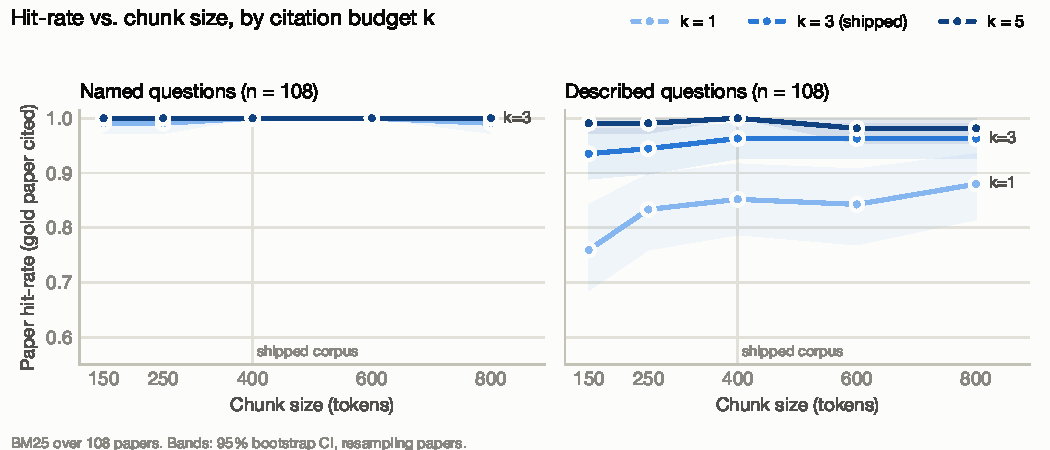
\includegraphics[width=\textwidth]{figures/ablation.pdf}
  \caption{Hit-rate vs.\ chunk size for $k = 1, 3, 5$. Left: questions that name their paper
    (at ceiling). Right: paraphrased questions. Shaded bands: 95\% paper-clustered bootstrap CIs.}
  \label{fig:ablation}
\end{figure}

\begin{table}[t]
  \centering\small
  \begin{tabular}{@{}lrr ccccc cc@{}}
    \toprule
    & & & \multicolumn{5}{c}{Described hit-rate at budget $k$} & \multicolumn{2}{c}{Terms in gold chunk} \\
    \cmidrule(lr){4-8}\cmidrule(l){9-10}
    Chunk size & Chunks & Median tok. & 1 & 2 & 3 & 4 & 5 & Described & Named \\
    \midrule
    150          & 14{,}310 & 133 & .759 & .861 & .935          & .963  & .991  & 46\% & 75\% \\
    250          &  8{,}770 & 226 & .833 & .926 & .944          & .963  & .991  & 52\% & 81\% \\
    \textbf{400} &  5{,}711 & 357 & .852 & .917 & \textbf{.963} & 1.000 & 1.000 & 56\% & 82\% \\
    600          &  3{,}980 & 519 & .843 & .944 & .963          & .972  & .981  & 58\% & 85\% \\
    800          &  3{,}081 & 692 & .880 & .954 & .963          & .972  & .981  & 61\% & 85\% \\
    \bottomrule
  \end{tabular}
  \caption{Described questions ($n{=}108$) by chunk size; bold is deployed. Named questions score
    ${\ge}.991$ at $k{=}1$ and $1.000$ at $k{\ge}2$ for every size. Last two columns: mean share of a
    question's search terms present in the gold paper's best-matching chunk.}
  \label{tab:ablation}
\end{table}

\textbf{Results.}
\begin{enumerate}
  \item \textbf{Named questions are at ceiling.} Hit-rate is ${\ge}0.991$ at $k{=}1$ and $1.000$
    at $k{\ge}2$ for every chunk size, so chunk size cannot matter for this style. It is also the
    style of the dev set.
  \item \textbf{The budget matters most.} On described questions at c400, going from $k{=}1$ to
    $k{=}3$ adds 11.1 points [5.6, 17.6]: 12 questions gained, none lost, McNemar $p = 0.0005$.
    This survives correction.
  \item \textbf{Chunk size matters only at $k{=}1$, and only for the smallest chunks.} Against
    c400 at $k{=}1$ (all 216 questions): c150 $\Delta = -5.1$ points [$-8.8$, $-0.9$], 15
    questions lost vs.\ 4 gained, $p = 0.019$, which does \emph{not} survive Bonferroni. The other
    sizes are within noise: c250 $-1.4$, c600 $-0.5$, c800 $+0.9$, all with CIs spanning zero.
    The rising $k{=}1$ line in Fig.~\ref{fig:ablation} (0.76 $\to$ 0.88) is mostly c150 being
    worse; from 250 tokens up it is flat within noise.
  \item \textbf{At the deployed $k{=}3$, all sizes are equivalent.} Every $\Delta$ vs.\ c400 lies
    between $-1.4$ and $0.0$ points, with all CIs inside [$-3.7$, $+1.4$], and at most 5 of 216
    questions change outcome. Any real chunk-size effect at $k{=}3$ is smaller than about 4
    points.
\end{enumerate}

\textbf{Mechanism.} If small chunks hurt because a paraphrase's words are spread across the
paper, then the share of question terms found in the gold paper's best chunk should shrink with
chunk size, and more for described than for named questions. It does (Table~\ref{tab:ablation}):
from c800 to c150 it falls from 61\% to 46\% for described questions and from 85\% to 75\% for
named ones, whose rare name term anchors the match anyway. At $k{=}1$, a distractor chunk that
packs in a few common terms can then outrank the gold paper. A larger $k$ lets the gold paper
back in at rank 2 or 3, which is why the budget dominates.

\textbf{Decision.} Keep 400-token chunks and $k{=}3$. No size beats c400 at the deployed budget,
and c150 is the only size that looks worse. We do not move to $k{=}5$, even though described
hit-rate reaches 1.000. Each extra paper adds an excerpt (a longer prompt, more distractors in
the middle) and a citation the answer may not use. Those costs are invisible to this metric.

\textbf{Limitations: what could overturn this.}
\begin{itemize}
  \item \textbf{Retrieval only.} Answer quality, the primary grade, was not compared across
    sizes. Larger chunks cost prompt length (four excerpts are ${\approx}1.4$k tokens at c400 and
    ${\approx}2.8$k at c800), and our 2{,}000-character excerpt cap truncates c600/c800 chunks,
    so an answer-quality comparison would need a larger cap.
  \item \textbf{Hit-rate only counts recall.} It cannot penalize the noise that a larger $k$ or
    longer chunks add, so the case against $k{=}5$ is a judgement, not a measurement.
  \item \textbf{AI-written questions, from abstracts.} Abstract wording favours the abstract's
    chunk, which a 150-token chunking splits. The c150 penalty may be smaller for questions about
    a paper's body.
  \item \textbf{One retriever.} Dense or hybrid retrieval matches paraphrases by meaning and could
    flatten the described curve.
\end{itemize}
All numbers regenerate in about two minutes, without a GPU, using the commands in
\code{ablation/README.md}.

% ======================================================================
\section{Memory design (R3)}

\todo{Memory section. The rubric (15 pts) asks: what we store, when we write, what we
deliberately refuse to store and why. Privacy reasoning counts.}

% Points worth covering (from the README, eval_dev.py and L14):
% - What is stored, and in what form. The harness checks memory by exact, case-insensitive
%   substring match in get_memory() AND in the answer of a new session, so wording matters.
% - Write policy: when a write happens, and from what. Writing only from the user's own turns
%   (never from retrieved text or model output) is the defence against memory poisoning (L14).
% - What is refused, and why: sensitive categories, and the must-not-store facts behind the
%   negative probes (a leak fails the binary gate).
% - Scope and isolation: user_id scopes memory, session_id scopes history. Each record already
%   keeps its session_id and turn (provenance; see TABot._memory).
% - Deletion and correction: reset_memory(); what happens when a fact changes.
% - Use at answer time, and the sycophancy risk of tailoring answers to what the user said (L14).

% ======================================================================
\section{AI-use disclosure}

\textbf{Tools.} Claude Code (Anthropic's coding agent, model Claude Opus 5.5) in VS Code.
\todo{Teammate: tools used for the memory part.}

\textbf{What the AI did.} It explained the assignment and how lectures L11--L14 apply. It wrote
the retrieval, prompt, generation, citation and error-handling code in \code{ta\_bot.py}, and
every script in \code{ablation/} (corpus rebuilds, evaluation, statistics, plot). It wrote all
216 ablation questions, from paper titles and abstracts, and drafted Sections~1--2 of this report.
We chose the ablation axis and the question-set approach. \todo{What you changed or wrote
yourselves.}

\textbf{How we verified.}
\begin{itemize}
  \item \textbf{Interface:} \code{eval\_dev.py -{}-mock}, plus a 10-case test of the contract (a
    dead, slow or HTTP-500 endpoint raises \code{TimeoutError}; three endpoint URL forms; session
    isolation; per-user memory API; invalid citations dropped).
  \item \textbf{Retrieval:} we read the excerpts retrieved for every dev turn, not just the score.
    This exposed the turn-1 miss that last-turn scoring hid.
  \item \textbf{Ablation:} the 400-token rebuild equals the shipped corpus chunk for chunk;
    \code{check\_questions.py} screens for name leaks and copying; \todo{N of 216 questions
    checked by hand, and what we found}.
  \item \textbf{Generation:} we ran the dev set, 20 sampled ablation questions and 4 behaviour
    probes on PACE with Llama-3.1-8B. Claude read all 44 answers, flagged the problems listed in
    Section~1, and compared the answers before and after the fixes.
    \todo{Confirm you read the answers too.}
\end{itemize}
We take responsibility for all submitted code and claims.

% Optional (up to 5 bonus points): a documented case where the LLM judge scored us wrongly,
% with evidence.

\end{document}
